\documentclass[11pt,a4paper]{article}
\usepackage[utf8]{inputenc}
\usepackage[T1]{fontenc}
\usepackage{textgreek}
\usepackage{amsmath}
\usepackage{booktabs}
\usepackage{hyperref}
\usepackage{multicol}
\usepackage{graphicx}
\usepackage[margin=2cm]{geometry}

\setlength{\columnsep}{1cm}

\title{\vspace{-0.5cm}\textit{SnapBind}: Lightweight CNN for Protein Binding Pocket Prediction}
\author{David Z Barth, Alexander Haas, Elias M Bruss}
\date{}

\begin{document}

\vspace{1cm}
\maketitle
\vspace{-0.3cm}

\begin{multicols}{2} 

\section{Challenge Tackled}
Accurate protein AI models are costly in time and computational resources. \textit{SnapBind} addresses these challenges by providing a lightweight architecture that maintains high performance while being efficient enough for local deployment.
We provide high-throughput protein screening, binding site localization, academic accessibility without proprietary platforms and a local computational pipeline integration.

\section{Methods}

\noindent \quad \textbf{Dataset:} 100k protein-ligand pairs from BindingDB plus 20k negative controls (Antibodies, structural proteins, nucleases). Binding sites defined by 5Å cutoff with binary residue annotation. \\

\noindent \quad \textbf{Architecture:} FastCNNBindingPredictor with 64-dim embeddings, 128-dim hidden layers, 0.1 dropout, handling 20-300 residue sequences.\\

\noindent \quad \textbf{Training:} Batch size 32, AdamW (lr=2e-4), focal loss (α=1, γ=2) for class imbalance, early stopping, Apple Silicon GPU acceleration.

\section{What Worked Well}

Data Acquisition and the Training Pipeline \\

Three-pass architecture: (1) Sequence-based CNN for druggability, (2) ESM embeddings for evolutionary context, (3) SMILES integration for small-molecule ligand-specific predictions.\\

\textbf{Efficiency:} 0.5M parameters enable consumer hardware deployment with rapid batch processing and local execution. \\

\textbf{Performance:} Stable training with effective class imbalance handling through focal loss and positive class weighting.

\begin{center}
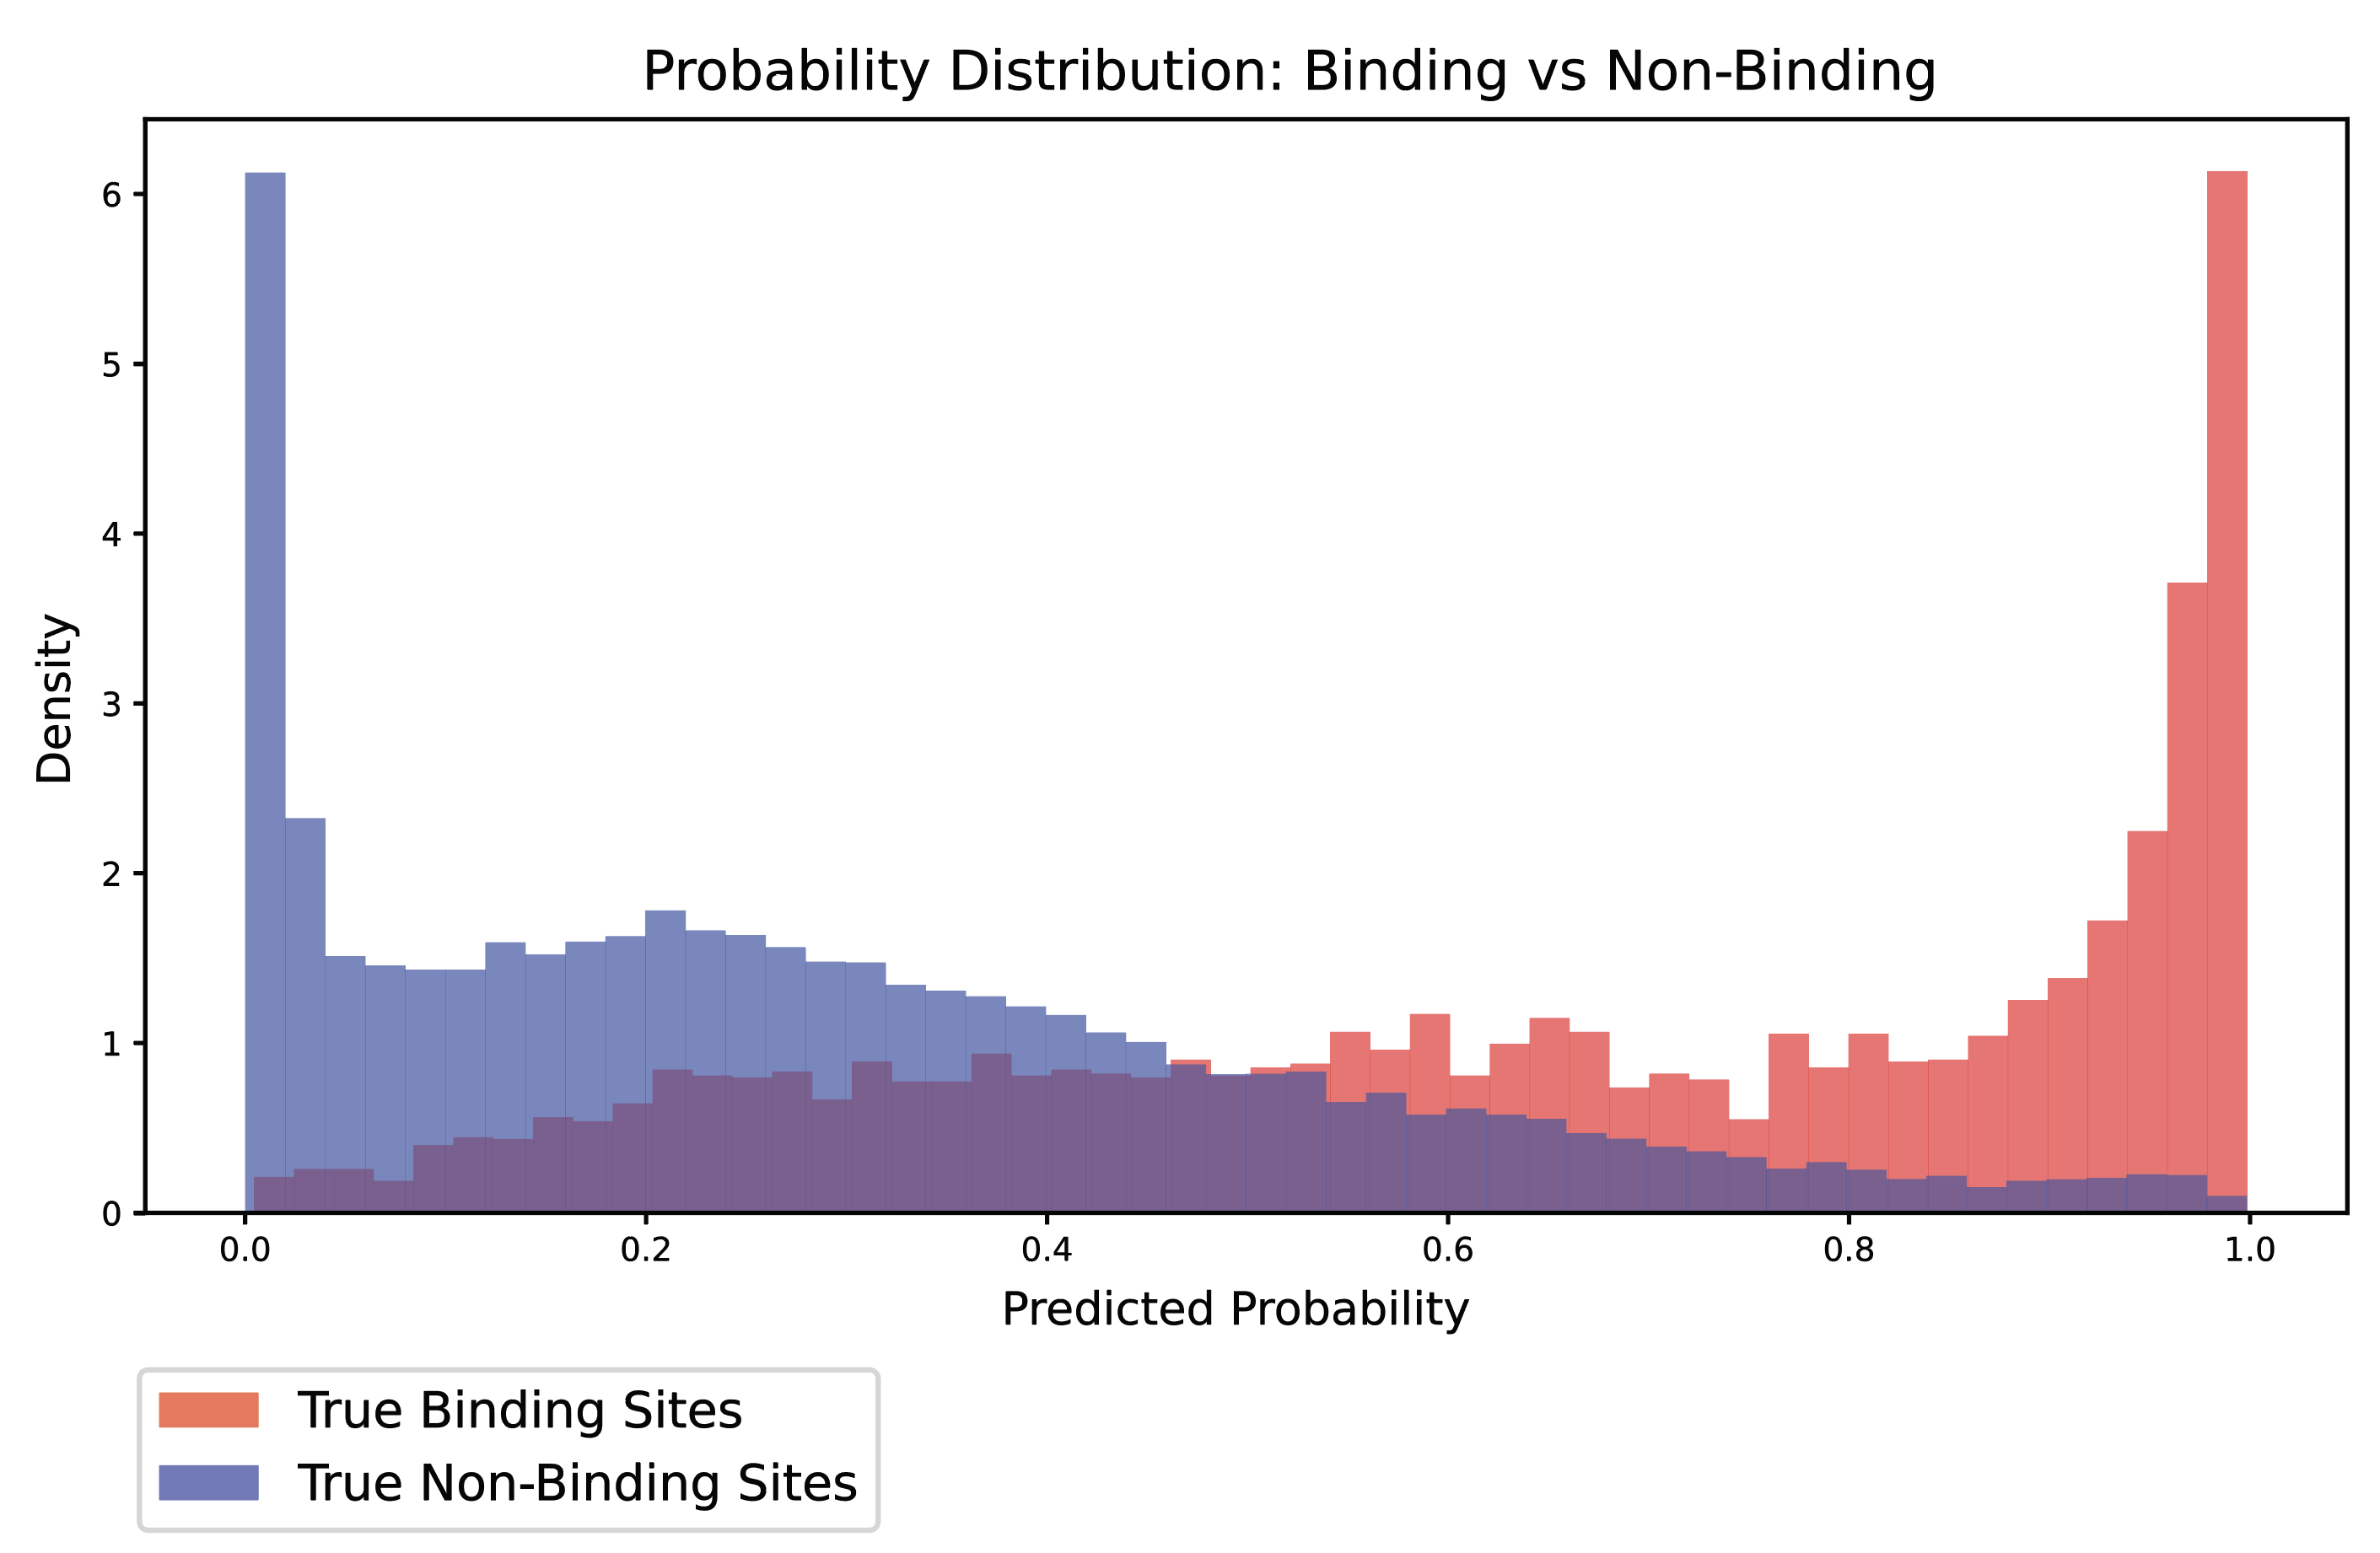
\includegraphics[width=1\columnwidth]{fig1mod.png}
\\[0.1cm]
\textbf{Figure 1:} Score distribution for ground truth.
\end{center}

\section{What Was Challenging}
Balancing model complexity with performance was a key challenge. While we aimed for a lightweight architecture, ensuring sufficient representational power to capture intricate protein-ligand interactions required careful design choices.

Front-end integration paired with a meaningful design philosophy required a lot of iterative refinement to achieve a user-friendly experience.

\section{Time Spent}
\begin{itemize}
    \item 0 - 1 h: Deciding on specific problem and first approach
    \item 1 - 5 h: Shared responsibilities - Data processing, different model architectures and benchmarking
    \item 5 - 10 h: Shared responsibilities - Model training, evaluation, and hyperparameter tuning, first steps towards integration
    \item 10 - 15 h: Shared responsibilities - Front-end integration, user interface design, and presentation
\end{itemize}


\section{Conclusion}

Our lightweight CNN democratizes binding pocket prediction by balancing performance with computational efficiency, enabling researchers to perform drug discovery screening without extensive infrastructure requirements.

\end{multicols}

\vfill

\end{document}
